\documentclass{ximera}

\newcommand{\RR}{\mathbb R}
\renewcommand{\d}{\,d}
\newcommand{\dd}[2][]{\frac{d #1}{d #2}}
\renewcommand{\l}{\ell}
\newcommand{\ddx}{\frac{d}{dx}}
\newcommand{\dfn}{\textbf}
\newcommand{\eval}[1]{\bigg[ #1 \bigg]}


\author{Jim Talamo and Alex Beckwith}
\license{Creative Commons 3.0 By-NC}


\outcome{Set up an integral that gives the length of a curve segment and evaluate it}

\begin{document}
\begin{exercise}

A cylindrical tank has base diameter 4m and height 10m. Suppose the tank is filled with water ($\rho$=1000 kg/m$^3$). Set up an integral that gives the work required to pump the water out of the tank then evaluate it.  Use $g=9.8$m/s$^2$.

\begin{image}
	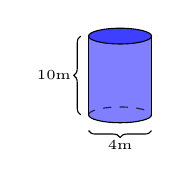
\begin{tikzpicture}
	
	\fill [blue,opacity=0.5] (0,0) ellipse (0.4 and 0.1);
	\fill [blue,opacity=0.5] (-0.4,0) -- (-0.4,-1) arc (180:360:0.4 and 0.1) -- (0.4,0) arc (0:180:0.4 and 0.1);
	
	\draw (0,0) ellipse (0.4 and 0.1);
	\draw (-0.4,0) -- (-0.4,-1);
	\draw (-0.4,-1) arc (180:360:0.4 and 0.1);
	\draw [dashed,opacity=0.75] (-0.4,-1) arc (180:360:0.4 and -0.1);
	\draw (0.4,-1) -- (0.4,0);  
	
	\draw[decoration={brace,raise=.1cm},decorate,thin] (-0.4,-1) -- (-0.4,0);
	\node[anchor=east] at (-0.5,-0.5) {\tiny $10$m};
	
	\draw[decoration={brace,raise=.1cm},decorate,thin] (0.4,-1.1) -- (-0.4,-1.1);
	\node[anchor=north] at (0,-1.2) {\tiny $4$m};

	\end{tikzpicture}
\end{image}

\[
W= \int_{y=\answer{0}}^{y=\answer{10}} \answer{39200\pi (10-y)}\d y = \answer[tolerance=10]{1960000\pi} J
\]
\begin{hint}
Set the height $y=0$ at the base of the tank.  We want to use the formula:

\[ 
W = \int_{y=0}^{y=b} \rho g A(y) d(y) \d y
\]

Since $b$ is the height to which the tank is filled, $b=\answer{10}$.

Since $h$ is the height to which the water must be moved, $h=\answer{10}$.

To move a slice to a height $y=10$, we find the distance $d(y)$ the slice at height $y$ must be moved is $d(y) = \answer{10-y}$

The cross-sectional area of this tank is:

\begin{multipleChoice}
\choice[correct]{is constant.}
\choice{varies depending on the height $y$ of the slice}.
\end{multipleChoice}

\begin{question}
Noting that the \emph{diameter} of the tank is given, the cross-sectional area is $A(y) = 2 \pi$.
\end{question}
\end{hint}
\end{exercise}
\end{document}
